\preClass{Coordinate Systems}



\noindent Watch the Pre-Class videos for Section 3.2 and answer the following questions. Remember that in your written work you are graded on the correctness of your supporting work and not just your final answer. Always give an exact answer unless you are explicitly told to round; calculator approximations will not receive full credit. 


\begin{enumerate}

\item  Graph the following functions.
\begin{enumerate}

\item  Graph $\displaystyle f(x)=\Big(\frac{1}{4}\Big)^x$ along with it's asymptote.  (It is helpful to plot values for $x=0, 1, -1$.)\\
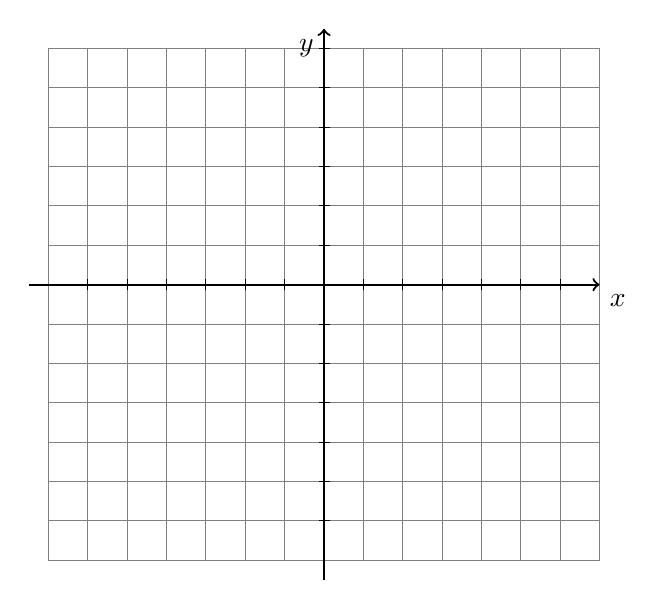
\begin{tikzpicture}[y=.5cm, x=0.5cm,font=\sffamily]
    %% ticks
    \draw[step = 1, gray] (-7,-7) grid (7,6);
    %% axis
    \draw[thick,->] (-7.5,0) -- coordinate (x axis mid) (7,0) node[anchor = north west] {$x$};
    \draw[thick,->] (0,-7.5) -- coordinate (y axis mid) (0,6.5) node[anchor = north east] {$y$};
    \foreach \y in {-6,-5,...,-1,1,2,...,6} {
      \draw (2pt, \y) -- (-2pt, \y);
    }
    \foreach \x in {-6,-5,...,-1,1,2,...,6} {
      \draw (\x,2pt) -- (\x,-2pt);
    }

\end{tikzpicture}



\item  Transform part $(a)$ to graph $\displaystyle g(x)=\Big(\frac{1}{4}\Big)^{x+3}-2$ along with it's asymptote.\\

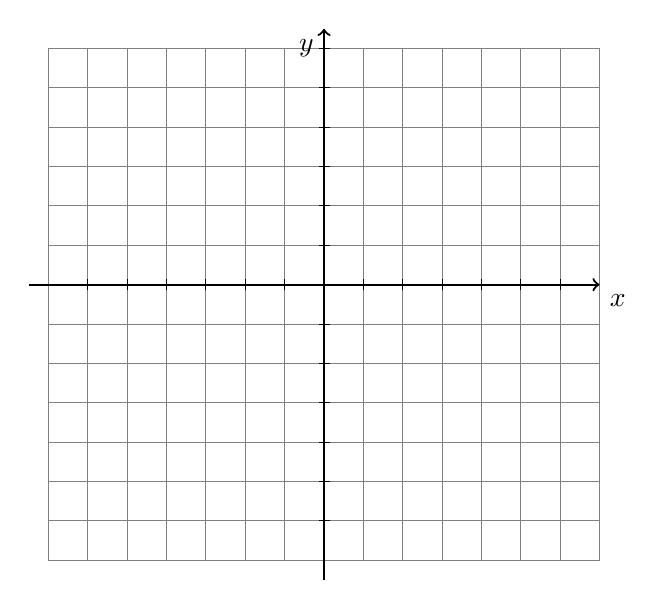
\begin{tikzpicture}[y=.5cm, x=0.5cm,font=\sffamily]
    %% ticks
    \draw[step = 1, gray] (-7,-7) grid (7,6);
    %% axis
    \draw[thick,->] (-7.5,0) -- coordinate (x axis mid) (7,0) node[anchor = north west] {$x$};
    \draw[thick,->] (0,-7.5) -- coordinate (y axis mid) (0,6.5) node[anchor = north east] {$y$};
    \foreach \y in {-6,-5,...,-1,1,2,...,6} {
      \draw (2pt, \y) -- (-2pt, \y);
    }
    \foreach \x in {-6,-5,...,-1,1,2,...,6} {
      \draw (\x,2pt) -- (\x,-2pt);
    }

\end{tikzpicture}


\vfill


\end{enumerate}



\vfill
\newpage

\item  Suppose that \$5000 is invested and pays 6.5\% per year under the following compounding options.  Determine the total amount in the account after 10 years with each option.

\begin{enumerate}
\item  Compounded monthly
\vfill
\item  Compounded continuously
\vfill

\end{enumerate}




\end{enumerate}



